\documentclass{article}
\usepackage[utf8]{vietnam}
\usepackage[OT1]{fontenc}
\usepackage[fontsize=13pt]{scrextend}
\usepackage[paperheight=29.7cm,paperwidth=21cm,right=2cm,left=3cm,top=2cm,bottom=2.5cm,twoside]{geometry}% Chuẩn A4, căn lề phải, trái, trên, dưới.
\usepackage{mathptmx}
\usepackage{amsmath}
\usepackage{graphicx} % Thư viện chèn ảnh
\usepackage{float} % Set vị trí chèn ảnh
\usepackage{tikz} % Thư viện tạo khung bìa
\usepackage{fontspec}
\setmonofont{Courier New}
\usetikzlibrary{calc} % Thư viện tikz
\usepackage{indentfirst} % Thư viện thụt đầu dòng
\usepackage{booktabs} % To thicken table lines
\usepackage{amssymb}

\renewcommand{\baselinestretch}{1.2} % Giãn dòng 1.2
\setlength{\parskip}{6pt} % Spacing after
\setlength{\parindent}{1cm} % Set khoảng cách thụt đầu dòng mỗi đoạn
\usepackage{titlesec} % Thư viện để set up các kiểu chữ
\usepackage{listings}
\usepackage{matlab-prettifier}
\setcounter{secnumdepth}{4} % 4 Heading
\titlespacing*{\section}{0pt}{0pt}{30pt} % Heading 1
\titleformat*{\section}{\fontsize{16pt}{0pt}\selectfont \bfseries \centering}

\titlespacing*{\subsection}{0pt}{10pt}{0pt} % Heading 2
\titleformat*{\subsection}{\fontsize{14pt}{0pt}\selectfont \bfseries}

\titlespacing*{\subsubsection}{0pt}{10pt}{0pt} % Heading 3
\titleformat*{\subsubsection}{\fontsize{13pt}{0pt}\selectfont \bfseries \itshape}

\titlespacing*{\paragraph}{0pt}{10pt}{0pt} % Heading 4
\titleformat*{\paragraph}{\fontsize{13pt}{0pt}\selectfont \itshape}

\renewcommand{\figurename}{\fontsize{12pt}{0pt}\selectfont \bfseries Figure}
\renewcommand{\thefigure}{\thesection.\arabic{figure}}
\usepackage[font=bf]{caption}
\captionsetup[figure]{labelsep=space}

\renewcommand{\tablename}{\fontsize{12pt}{0pt}\selectfont \bfseries Table}
\renewcommand{\thetable}{\thesection.\arabic{table}}
\captionsetup[table]{labelsep=space}

\usepackage{tabularx}
\newcolumntype{s}{>{\hsize=.3\hsize}X}
\newcolumntype{y}{>{\hsize=.4\hsize}X}
\newcolumntype{d}{>{\hsize=.1\hsize}X}
\newcolumntype{a}{>{\hsize=1.1\hsize}X}
\newcolumntype{g}{>{\hsize=5\hsize}X}
\renewcommand{\tabularxcolumn}[1]{>{\small}m{#1}}

\renewcommand{\theequation}{\thesection.\arabic{equation}} % Thay đổi đánh số phương trình mặc định
\newtheorem{theorem}{Định lý}[section]
\newtheorem{defn}[theorem]{Định nghĩa}
\newtheorem{corollary}[theorem]{Hệ quả}
\newtheorem{lemma}[theorem]{Bổ đề}
\usepackage{lipsum} % Thư viện tạo chữ linh tinh.

\usepackage[unicode]{hyperref}
\usepackage{colortbl}
\definecolor{LightCyan}{rgb}{0.88,1,1}
\usepackage{forloop}
\newcounter{loopcntr}
\newcommand{\rpt}[2][1]{\forloop{loopcntr}{0}{\value{loopcntr}<#1}{#2}}

\begin{document}
	\setmainfont{Times New Roman}
	\thispagestyle{empty}
	\begin{center}
		\vspace{-12pt}  \fontsize{14pt}{0pt}\selectfont ĐẠI HỌC BÁCH KHOA HÀ NỘI \\[6pt]
		\textbf{\fontsize{16pt}{0pt}\selectfont TRƯỜNG ĐIỆN - ĐIỆN TỬ}
		\vspace{1.75cm}
		\begin{figure}[H]
			\centering
			
\includegraphics[height=4.25cm]{logoHUST.png}
		\end{figure}
		\vspace{1cm}
		\textbf{\fontsize{25pt}{0pt}\selectfont ĐỒ ÁN THIẾT KẾ I} 
		\vspace{0.5cm}
	\end{center}
	\begin{center}
		\textbf{\fontsize{22pt}{0pt}\selectfont Xây dựng website hỗ trợ học tập} \\
		\vspace{2.5cm}
		
		\textbf{\fontsize{18pt}{0pt}\selectfont ĐẶNG QUANG VŨ} \\[6pt]
		\fontsize{16pt}{0pt}\selectfont vu.dq223830@sis.hust.edu.vn \\[6pt]
		\vspace{0.75cm}
		\textbf{\fontsize{16pt}{0pt}\selectfont Ngành Điện tử - Viễn thông} \\[6pt]
		\textbf{\fontsize{16pt}{0pt}\selectfont Chuyên ngành Kỹ thuật Điện tử - Viễn thông} 
		\vspace{0.75cm}
		\begin{table}[H]
			\centering
			\begin{tabular}{l l l}
				\fontsize{16pt}{0pt}\selectfont \textbf{Giảng viên hướng dẫn:}    & \fontsize{16pt}{0pt}\selectfont ThS. Đinh Thị Nhung \vspace{6pt} & \_\_\_\_\_\_\_\_\_\_\_ \\ 
			\end{tabular}
		\end{table}
		\vspace{2.5cm}
		\fontsize{14pt}{0pt}\selectfont \textbf{Hà Nội, 6/2025}
	\end{center}
	\cleardoublepage
	\thispagestyle{empty}
	\begin{center}
		\vspace{-12pt}  \fontsize{14pt}{0pt}\selectfont ĐẠI HỌC BÁCH KHOA HÀ NỘI \\[6pt]
		\textbf{\fontsize{16pt}{0pt}\selectfont TRƯỜNG ĐIỆN - ĐIỆN TỬ}
		\vspace{1.75cm}
		\begin{figure}[H]
			\centering
			
\includegraphics[height=4.25cm]{logoHUST.png}
		\end{figure}
		\vspace{1cm}
		\textbf{\fontsize{25pt}{0pt}\selectfont ĐỒ ÁN THIẾT KẾ I} 
		\vspace{0.5cm}
	\end{center}
	\begin{center}
		\textbf{\fontsize{22pt}{0pt}\selectfont Xây dựng website hỗ trợ học tập} \\
		\vspace{2.5cm}
		
		\textbf{\fontsize{18pt}{0pt}\selectfont ĐẶNG QUANG VŨ} \\[6pt]
		\fontsize{16pt}{0pt}\selectfont vu.dq223830@sis.hust.edu.vn \\[6pt]
		\vspace{0.75cm}
		\textbf{\fontsize{16pt}{0pt}\selectfont Ngành Điện tử - Viễn thông} \\[6pt]
		\textbf{\fontsize{16pt}{0pt}\selectfont Chuyên ngành Kỹ thuật Điện tử - Viễn thông} 
		\vspace{0.75cm}
		\begin{table}[H]
			\centering
			\begin{tabular}{l l l}
				\fontsize{16pt}{0pt}\selectfont \textbf{Giảng viên hướng dẫn:}    & \fontsize{16pt}{0pt}\selectfont ThS. Đinh Thị Nhung \vspace{6pt} &  \\ 
			\end{tabular}
		\end{table}
		\vspace{2.5cm}
		\fontsize{14pt}{0pt}\selectfont \textbf{Hà Nội, 6/2025}
	\end{center}
	\cleardoublepage
	\section*{LỜI NÓI ĐẦU}
	\thispagestyle{empty}
	Trong thời đại số hóa hiện nay, việc truy cập và sử dụng tài liệu học tập, nghiên cứu, cũng như các tài liệu chuyên ngành ngày càng trở nên thiết yếu đối với sinh viên. Tài liệu không chỉ là nguồn cung cấp kiến thức nền tảng, mà còn là công cụ hỗ trợ hiệu quả cho việc cập nhật kiến thức mới, rèn luyện kỹ năng tư duy phản biện, và thúc đẩy quá trình học tập.
	
	Tuy nhiên, cùng với sự bùng nổ về số lượng và chủng loại tài liệu, người dùng lại đối mặt với nhiều thách thức trong việc tìm kiếm, chọn lọc và truy cập tài liệu một cách hiệu quả. Các nền tảng tài liệu hiện nay thường phân tán trên nhiều hệ thống khác nhau, thiếu tính liên kết và đồng bộ. Trong khi một số hệ thống bị giới hạn phạm vi truy cập (chỉ dành cho một nhóm đối tượng cụ thể như sinh viên trong trường hoặc người có trả phí cao), thì các nền tảng mở lại thiếu sự tổ chức, kiểm duyệt và phân loại rõ ràng, gây nhiễu thông tin và ảnh hưởng đến trải nghiệm người dùng.
	
	Bên cạnh đó, không phải ai cũng có cùng một trình độ chuyên môn hoặc nhu cầu sử dụng tài liệu như nhau. Một hệ thống tài liệu lý tưởng cần phải phân tầng truy cập thông minh, cho phép người dùng ở các cấp độ (như người mới bắt đầu, người học nâng cao, hay chuyên gia) có thể tiếp cận với loại tài liệu phù hợp với trình độ và mục tiêu học tập của mình. Điều này không chỉ giúp tối ưu hóa trải nghiệm học tập, mà còn góp phần đảm bảo tính bảo mật, quản lý tốt hơn quyền truy cập và tránh lãng phí tài nguyên.
	
	Xuất phát từ những nhu cầu thực tiễn trên, việc xây dựng một hệ thống hỗ trợ quản lý và truy cập tài liệu học thuật và chuyên ngành theo hướng hiệu quả, có tổ chức và phân quyền rõ ràng là hết sức cần thiết. Đây sẽ là công cụ quan trọng nhằm kết nối người học với nguồn tài liệu giá trị, tạo điều kiện thúc đẩy việc học tập chủ động, phát triển năng lực cá nhân, đồng thời hỗ trợ tốt hơn cho các hoạt động giảng dạy và nghiên cứu trong môi trường học thuật hiện đại.
	\cleardoublepage
	
	\addtocontents{toc}{\protect\thispagestyle{empty}}
	\renewcommand{\contentsname}{MỤC LỤC}
	\tableofcontents 
	\thispagestyle{empty}
	\cleardoublepage
	
	\pagenumbering{roman} % Đánh số thứ tự la mã
	\section*{DANH MỤC KÝ HIỆU VÀ CHỮ VIẾT TẮT}
	\phantomsection \addcontentsline{toc}{section}{\numberline {} DANH MỤC KÝ HIỆU VÀ CHỮ VIẾT TẮT}
	
	\begin{tabular}{ l l }
		\hspace{1cm} AWGN & \hspace{4cm} Additive White Gaussian Noise \\  
		\hspace{1cm} BC & \hspace{4cm} Broadcast Channel    \\
		\hspace{1cm} BS  & \hspace{4cm} Base Station\\
		\hspace{1cm} CSI & \hspace{4cm} Channel State Information \\  
	\end{tabular}  
	
	\newpage
	
	\renewcommand{\listfigurename}{DANH MỤC HÌNH VẼ}
	{\let\oldnumberline\numberline
		\renewcommand{\numberline}{Hình~\oldnumberline}
		\listoffigures} 
	\phantomsection\addcontentsline{toc}{section}{\numberline {} DANH MỤC HÌNH VẼ}
	\newpage
	
	%Tạo danh mục bảng biểu.
	\renewcommand{\listtablename}{DANH MỤC BẢNG BIỂU}
	{\let\oldnumberline\numberline
		\renewcommand{\numberline}{Bảng~\oldnumberline}
		\listoftables}
	\phantomsection\addcontentsline{toc}{section}{\numberline {} DANH MỤC BẢNG BIỂU}
	\newpage
	
	\section*{TÓM TẮT ĐỒ ÁN}
	\phantomsection\addcontentsline{toc}{section}{\numberline {}TÓM TẮT ĐỒ ÁN}
	Trong bối cảnh số hóa mạnh mẽ hiện nay, nhu cầu truy cập và khai thác tài liệu học tập, nghiên cứu ngày càng gia tăng. Tuy nhiên, việc phân tán tài liệu trên nhiều nền tảng, thiếu tính tổ chức và không phân quyền truy cập hợp lý khiến người dùng gặp khó khăn trong việc tìm kiếm, sử dụng tài nguyên hiệu quả. Đồ án này đề xuất và xây dựng một hệ thống quản lý và chia sẻ tài liệu học tập có tổ chức, hỗ trợ người dùng ở nhiều cấp độ khác nhau (cơ bản, nâng cao, chuyên sâu). Hệ thống cho phép người dùng đăng tải, tìm kiếm, truy cập và tải về tài liệu một cách dễ dàng, đồng thời có cơ chế phân quyền để kiểm soát truy cập phù hợp với nhu cầu và trình độ người dùng. Giải pháp này nhằm tối ưu hóa quá trình học tập, chia sẻ tri thức và nâng cao hiệu quả khai thác tài liệu số.
	
	\vspace{2cm}
	
	\section*{ABSTRACT}
	In today's rapidly digitalized world, the demand for accessing and utilizing educational and research materials is steadily increasing. However, the fragmentation of resources across various platforms, along with a lack of structure and appropriate access control, often hinders users from efficiently finding and using valuable content. This project introduces and develops an organized document management and sharing system that supports users at different proficiency levels (basic, intermediate, advanced). The system enables users to upload, search, access, and download documents with ease, while implementing access control mechanisms to ensure that materials are delivered according to users’ needs and expertise levels. This solution aims to optimize the learning process, facilitate knowledge sharing, and enhance the efficiency of digital resource utilization.
	\cleardoublepage
	
	\pagenumbering{arabic} % Đánh số thứ tự 1,2,3...
	\section*{CHƯƠNG 1. TỔNG QUAN ĐỀ TÀI}
	\addcontentsline{toc}{section}{\numberline{}CHƯƠNG 1. TỔNG QUAN ĐỀ TÀI}
	\setcounter{section}{1}
	\setcounter{subsection}{0}
	\setcounter{figure}{0}
	\setcounter{table}{0}
	
	Chương này sẽ trình bày về tổng quan tình hình nghiên cứu, lý do chọn đề tài,phương pháp được chọn để thực hiện đề tài, mục tiêu đề tài cần phải đạt được.
	
	\subsection{Đặt vấn đề}
	
	Trong những năm gần đây, cùng với sự phát triển mạnh mẽ của công nghệ thông tin và Internet, quá trình học tập và nghiên cứu đang dần dịch chuyển sang môi trường số hóa. Tài liệu học tập, tài liệu nghiên cứu và các nguồn tri thức khác được số hóa và lưu trữ ngày càng nhiều trên các nền tảng trực tuyến. Điều này mang lại cơ hội lớn cho người học và người làm công tác nghiên cứu tiếp cận nhanh chóng và tiện lợi với kho tri thức toàn cầu.
	
	Tuy nhiên, bên cạnh những thuận lợi, thực tế cũng đặt ra nhiều thách thức. Khối lượng tài liệu số ngày càng đồ sộ, nhưng lại thiếu sự tổ chức hợp lý, gây khó khăn cho việc tra cứu, chọn lọc và sử dụng hiệu quả. Nhiều hệ thống tài liệu hiện tại chỉ phục vụ trong nội bộ (ví dụ như thư viện số của một trường đại học), trong khi các hệ thống mở lại thiếu tính kiểm soát và phân loại rõ ràng. 
	
	Chính vì vậy, việc xây dựng một hệ thống hỗ trợ quản lý, chia sẻ và truy cập tài liệu học tập dễ sử dụng là rất cần thiết. Hệ thống cần giải quyết đồng thời nhiều yêu cầu như: cho phép người dùng đóng góp tài liệu, tìm kiếm nhanh chóng. Điều này không chỉ giúp tiết kiệm thời gian và công sức trong việc tra cứu tài liệu, mà còn góp phần nâng cao chất lượng học tập, nghiên cứu và chia sẻ tri thức một cách có định hướng.
	
	Từ những lý do trên, nhóm thực hiện đồ án đã lựa chọn đề tài: \textbf{\textit{"Xây dựng website hỗ trợ học tập"}} nhằm giải quyết những vấn đề thực tiễn đang tồn tại, đồng thời đóng góp một công cụ hữu ích cho cộng đồng học tập và nghiên cứu.
	
	\subsection{Mục đích nghiên cứu}
	
	Mục đích chính của đề tài là xây dựng một hệ thống quản lý và chia sẻ tài liệu học tập có tổ chức, hiệu quả và dễ sử dụng, nhằm hỗ trợ người dùng ở nhiều cấp độ (từ cơ bản đến nâng cao) trong việc tiếp cận và khai thác tài nguyên tri thức một cách thuận tiện, nhanh chóng và phù hợp với nhu cầu.
	
	Cụ thể, đề tài hướng đến các mục tiêu sau:

	\begin{itemize}
		\item Thiết kế và phát triển hệ thống web hỗ trợ lưu trữ, phân loại, tìm kiếm và chia sẻ tài liệu học tập, nghiên cứu hoặc chuyên ngành một cách khoa học và dễ sử dụng.
		\item Tạo điều kiện cho người dùng đóng góp tài liệu, với quy trình kiểm duyệt hợp lý nhằm đảm bảo chất lượng nội dung, tính chính xác và phù hợp với định hướng học thuật.
		\item Góp phần xây dựng một nền tảng học tập mở nhưng có tổ chức, giúp nâng cao hiệu quả tự học, tiết kiệm thời gian tìm kiếm tài liệu, đồng thời tạo môi trường học thuật cộng tác và chia sẻ kiến thức lành mạnh.
	\end{itemize}
	
	\subsection{Kết luận chương}
	
	Tóm lại, trước những bất cập trong việc truy cập và sử dụng tài liệu hiện nay, việc xây dựng một hệ thống hỗ trợ, quản lý tài liệu học tập là hết sức cần thiết. Đề tài đã xác định được mục tiêu, phạm vi và định hướng phát triển hệ thống nhằm hỗ trợ người dùng hiệu quả hơn trong quá trình học tập và nghiên cứu. Để triển khai hệ thống một cách khoa học, chương tiếp theo sẽ trình bày các cơ sở lý thuyết liên quan làm nền tảng cho quá trình phân tích và thiết kế hệ thống.
	\newpage
	
	\section*{CHƯƠNG 2. CƠ SỞ LÝ THUYẾT}
	\addcontentsline{toc}{section}{\numberline{}CHƯƠNG 2. CƠ SỞ LÝ THUYẾT}
	\setcounter{section}{2}
	\setcounter{subsection}{0}
	\setcounter{figure}{0}
	\setcounter{table}{0}
	
	Chương này sẽ trình bày những kiến thức nền tảng liên quan đến hệ thống quản lý tài liệu, phân quyền người dùng, mô hình kiến trúc phần mềm, cũng như các công nghệ được sử dụng trong việc thiết kế và phát triển hệ thống. Những cơ sở lý thuyết này sẽ giúp đảm bảo hệ thống được triển khai đúng hướng, đáp ứng tốt các yêu cầu đặt ra về chức năng, hiệu năng và bảo mật.
	
	\subsection{Mô hình MVC}
	
	Mô hình MVC (Model-View-Controller) là một mẫu kiến trúc phần mềm phổ biến được sử dụng trong phát triển ứng dụng web, giúp phân chia ứng dụng thành ba thành phần chính: Model, View, và Controller được biểu diễn trên Hình \ref{fig21}. Mỗi thành phần đảm nhận một vai trò riêng, giúp tăng tính tổ chức, khả năng bảo trì và mở rộng của ứng dụng. 
	
	\begin{figure}[!ht]
		\centering
		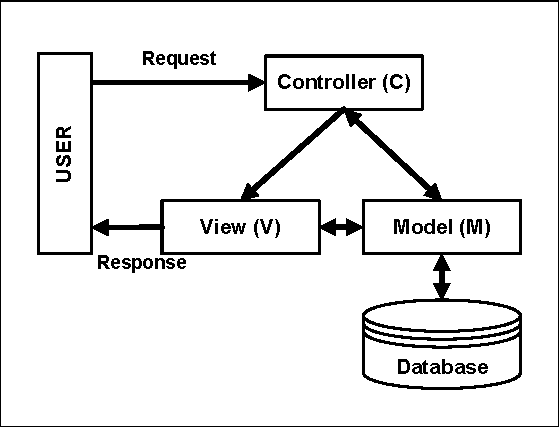
\includegraphics[trim= 10pt 10pt 10pt 10pt, clip, width=8cm]{mvc_fig21.pdf}
		\caption[Mô hình MVC]{\bfseries \fontsize{12pt}{0pt}\selectfont Mô hình MVC}
		\label{fig21}
	\end{figure}
	
	\textbf{Model:} Đây là thành phần chịu trách nhiệm xử lý dữ liệu và logic nghiệp vụ. Model quản lý trạng thái của dữ liệu, tương tác với cơ sở dữ liệu (chẳng hạn như MySQL, SQL Server, SQLite, ...), và thực hiện các thao tác như thêm, sửa, xóa hoặc truy vấn thông tin tài liệu, người dùng, v.v...
	
	\textbf{View:} Thành phần này đại diện cho giao diện người dùng - nơi người dùng tương tác trực tiếp với hệ thống. Trong đề tài, phần View được phát triển bằng ReactJS, hiển thị các dữ liệu như danh sách tài liệu, thông tin chi tiết, giao diện đăng nhập, đăng ký, phân quyền, v.v... View nhận dữ liệu từ Controller và hiển thị lại cho người dùng theo cách trực quan, dễ sử dụng.
	
	\textbf{Controller:} Controller đóng vai trò trung gian giữa Model và View. Nó tiếp nhận các yêu cầu từ người dùng thông qua View (chẳng hạn như thao tác đăng nhập, tìm kiếm tài liệu, tải lên file), xử lý yêu cầu đó bằng cách tương tác với Model, sau đó trả kết quả lại cho View để hiển thị. Trong hệ thống này, Controller được cài đặt ở backend thông qua Node.js và Express, đóng vai trò định tuyến và xử lý logic của ứng dụng.
	
	Việc áp dụng mô hình MVC giúp hệ thống được chia tách rõ ràng theo chức năng, giúp dễ dàng mở rộng, tái sử dụng mã nguồn, và thuận tiện cho việc phát triển theo nhóm hoặc bảo trì lâu dài. Đây là một kiến trúc phù hợp cho các ứng dụng web hiện đại, đặc biệt là các hệ thống có quy mô vừa và lớn.
\end{document}